%===================== RESULTADOS E DISCUSSÃO =====================
\section{Resultados e discussão}

\subsection{Métricas de desempenho do modelo}
\label{subsec:metricas-modelo}

Os resultados a seguir foram obtidos com um \textit{dataset} inicial de 2 classes
de gestos (``oi'' e ``obrigado''), após a aplicação dos critérios de exclusão
descritos na Seção~\ref{subsec:coleta}. A Tabela~\ref{tab:metricas} apresenta as
métricas por classe sobre o conjunto de teste.

% [PENDENTE: conferir os números do dataset: o protocolo prevê 10 participantes ×
% 10 repetições (>= 100 amostras por gesto), a versão anterior citava
% "aproximadamente 30 amostras por gesto", e o suporte da tabela soma 38. Informar
% o total de amostras por gesto após a exclusão e quantas foram para treino,
% validação e teste.]

\begin{table}[htbp]
\centering
\caption{Métricas de classificação por classe no conjunto de teste.}
\label{tab:metricas}
\begin{tabular}{@{}l c c c c@{}}
\toprule
\textbf{Gesto} & \textbf{Precisão} & \textbf{Revocação} & \textbf{F1-score} & \textbf{Suporte} \\
\midrule
obrigado & 1,00 & 0,93 & 0,96 & 14 \\
oi & 0,96 & 1,00 & 0,98 & 24 \\
\midrule
Média macro & 0,98 & 0,96 & 0,97 & 38 \\
\addlinespace
\multicolumn{4}{@{}l}{Acurácia global} & 97,4\% \\
\multicolumn{4}{@{}l}{Kappa de Cohen} & 0,94 \\
\bottomrule
\end{tabular}
\end{table}

Complementarmente, o modelo obteve F1 macro de 0,97 e coeficiente Kappa de Cohen
de 0,94, indicando concordância quase perfeita entre as predições do modelo e os
rótulos reais: segundo a escala de interpretação de Landis e Koch (1977), valores
de Kappa entre 0,81 e 1,00 correspondem a concordância quase perfeita.

\begin{figure}[htbp]
\centering
\figpendente{Inserir a imagem gerada por \texttt{evaluate\_model.py} (pasta
\texttt{logs/} ou equivalente).}
\caption{Matriz de confusão do modelo no conjunto de teste.}
\label{fig:cm-modelo}
\end{figure}

\begin{figure}[htbp]
\centering
\figpendente{Inserir o gráfico gerado a partir do \texttt{CSVLogger}
(\texttt{logs/training\_log.csv} ou equivalente).}
\caption{Curvas de acurácia e perda de treinamento e validação ao longo das
épocas.}
\label{fig:curvas}
\end{figure}

\subsection{Discussão dos resultados}

O resultado de 97,4\% de acurácia é expressivo e está em linha com trabalhos
recentes da área — a título de comparação, o sistema de reconhecimento de sílabas
em Libras listado na Tabela~\ref{tab:relacionados} reporta exatamente o mesmo
valor de acurácia média em condições controladas, ainda que sobre vocabulário e
\textit{dataset} distintos. Também é superior ao reportado por Rego et al.\ (2025)
no \textit{dataset} MINDS-Libras (92\%), embora essa comparação deva ser lida com
cautela, pois os \textit{datasets}, o número de classes e a metodologia de
validação não são idênticos.

É necessário, no entanto, interpretar esse número com cautela metodológica. O
conjunto avaliado contém apenas 2 classes e 38 amostras de teste — uma base de
dados consideravelmente menor do que a de trabalhos de referência da área, como o
MINDS-Libras, que reúne 1.155 vídeos cobrindo 20 sinais executados por 12
sinalizantes (REZENDE; ALMEIDA; GUIMARÃES, 2021). \textit{Datasets} pequenos
aumentam o risco de \textit{overfitting}: é possível que o modelo esteja
memorizando particularidades dos poucos sinalizantes presentes no treinamento, em
vez de aprender um padrão de gesto generalizável. Esse risco é discutido de forma
mais detalhada na Seção~\ref{subsec:limitacoes}.

Com a ampliação planejada do \textit{dataset} — para 60 a 100 amostras por gesto,
maior número de participantes e inclusão de vocabulário relacionado à área de
computação (ver Seção~\ref{subsec:futuros}) — espera-se manter ou aproximar essa
acurácia sob condições de avaliação mais rigorosas, notadamente com validação em
dados de usuários não presentes no treinamento.

\subsection{Dados coletados na plataforma web}

Até a data desta versão, a plataforma registra 6 participantes cadastrados, dos
quais 4 contribuíram com gravações, todas realizadas entre 2 e 4 de junho de
2026. A Tabela~\ref{tab:composicao} resume o \textit{dataset} exportado, e a
Figura~\ref{fig:quadros-part} mostra a contribuição de cada participante.

\begin{table}[htbp]
\centering
\caption{Composição do dataset da plataforma web.}
\label{tab:composicao}
\begin{tabular}{@{}l c@{}}
\toprule
\textbf{Item} & \textbf{Valor} \\
\midrule
Participantes cadastrados & 6 \\
Participantes com gravações & 4 \\
Participantes com deficiência auditiva declarada & 0 \\
Gravações (gesto $\times$ participante) & 30 \\
Gestos distintos & 23 \\
Gestos gravados por mais de um participante & 5 (A, B, C, E, L) \\
Quadros brutos (até 150 por gravação) & 3.481 \\
Quadros amostrados para o classificador & 597 \\
\bottomrule
\end{tabular}
\end{table}

Cada gesto de cada participante corresponde a uma única gravação; as ``20
amostras'' exibidas na plataforma são quadros dessa gravação, e não repetições
independentes do gesto. Por isso, o \textit{dataset} ainda não atende ao
protocolo de 10 repetições por gesto descrito na Seção~\ref{subsec:coleta}.

\begin{figure}[htbp]
\centering
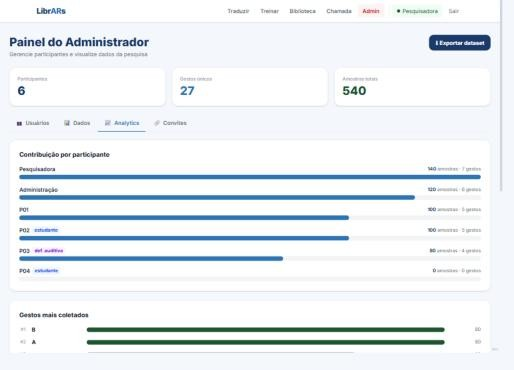
\includegraphics[width=0.75\textwidth]{fig_contribuicao}
\caption{Quadros amostrados e gestos gravados por participante.}
\label{fig:quadros-part}
\end{figure}

\subsection{Avaliação do classificador da plataforma web}

O classificador descrito na Seção~\ref{subsec:classificador-plataforma} foi
avaliado sobre o \textit{dataset} exportado, reproduzindo a mesma regra de decisão
e os mesmos limiares usados em produção. A avaliação é feita por quadro e
considera três desfechos: acerto, erro (outro gesto aceito) ou rejeição. Foram
usados dois cenários:

\begin{itemize}[leftmargin=2cm]
  \item \textbf{Mesmo sinalizante:} para as 19 gravações do participante P01, a
  primeira metade dos quadros de cada gravação serve de referência e a segunda
  metade é classificada. Como os quadros vêm da mesma gravação, este cenário é
  otimista;
  \item \textbf{Sinalizante excluído} (\textit{leave-one-participant-out}): os
  quadros de cada participante são classificados usando como referência apenas as
  gravações dos demais. Só entram os gestos que outro participante também gravou
  (A, B, C, E e L).
\end{itemize}

\begin{table}[htbp]
\centering
\caption{Desempenho do classificador da plataforma, por quadro.}
\label{tab:desempenho-plataforma}
\begin{tabular}{@{}l c c@{}}
\toprule
 & \textbf{Mesmo sinalizante} & \textbf{Sinalizante excluído} \\
\midrule
Quadros avaliados & 1.383 & 1.319 \\
Gestos & 19 & 5 \\
Acertos & 72,5\% & 35,5\% \\
Erros & 13,5\% & 9,9\% \\
Rejeitados & 14,0\% & 54,7\% \\
Precisão entre os aceitos & 84,3\% & 78,3\% \\
\bottomrule
\end{tabular}
\end{table}

No cenário de mesmo sinalizante (Figura~\ref{fig:cm-mesmo}), 11 dos 19 gestos
superam 85\% de acerto. As falhas se concentram em pares de configuração de mão
semelhante: B é confundido com F, S com MULHER e V com U; C, E e L são
majoritariamente rejeitados.

Com o sinalizante excluído (Figuras~\ref{fig:cm-excluido} e~\ref{fig:acerto-part}),
o acerto cai para 35,5\%, e a maior parte dos quadros é rejeitada, e não
classificada errado: o classificador tende a abster-se diante de uma mão que não
conhece. A exceção é a letra A, confundida com MULHER em 43\% dos quadros. O
desempenho também varia muito entre participantes, de 0\% a 82\%.

\begin{figure}[htbp]
\centering
\figpendente{Matriz de confusão do classificador da plataforma no cenário de
mesmo sinalizante (participante P01).}
\caption{Matriz de confusão do classificador da plataforma no cenário de mesmo
sinalizante (participante P01).}
\label{fig:cm-mesmo}
\end{figure}

\begin{figure}[htbp]
\centering
\figpendente{Matriz de confusão no cenário de sinalizante excluído.}
\caption{Matriz de confusão no cenário de sinalizante excluído.}
\label{fig:cm-excluido}
\end{figure}

\begin{figure}[htbp]
\centering
\figpendente{Gráfico de barras: acerto por participante no cenário de sinalizante
excluído.}
\caption{Acerto por participante no cenário de sinalizante excluído.}
\label{fig:acerto-part}
\end{figure}

Por fim, os 2.162 quadros de gestos que não existiam na referência do cenário de
sinalizante excluído permitem medir o comportamento diante de sinais
desconhecidos: 77,8\% foram corretamente rejeitados, mas 22,2\% foram aceitos
como algum outro gesto.

Esses resultados confirmam, com dados reais da plataforma, a limitação de
generalização discutida na Seção~\ref{subsec:limitacoes}: o reconhecimento
funciona bem para quem gravou o gesto, mas ainda não para novos usuários. A
avaliação considera apenas o caminho estático do classificador e quadros
isolados; o desempenho percebido na tela Traduzir, que acumula decisões ao longo
do tempo, pode ser diferente.

\subsection{Resultados da validação com usuários}

% [PENDENTE: seção a ser preenchida após as sessões descritas na
% Seção 4.6. Conteúdo previsto: tabela de caracterização dos participantes
% (anonimizada), acurácia por participante, matriz de confusão agregada, tempo
% médio até o reconhecimento e síntese do questionário de percepção.]

\begin{figure}[htbp]
\centering
\figpendente{Gráfico de barras: participantes P01–P05 no eixo $x$, acurácia no
eixo $y$, com linha de referência na acurácia do conjunto de teste original.}
\caption{Acurácia de reconhecimento por participante na validação.}
\label{fig:acuracia-validacao}
\end{figure}

\begin{figure}[htbp]
\centering
\figpendente{Gráfico de barras empilhadas por item do questionário (escala de 1 a
5).}
\caption{Respostas ao questionário de percepção.}
\label{fig:questionario}
\end{figure}

\subsection{Limitações}
\label{subsec:limitacoes}

Apesar dos resultados preliminares expressivos, este trabalho apresenta
limitações que devem ser consideradas na interpretação dos resultados e no
planejamento das próximas etapas:

\begin{itemize}[leftmargin=2cm]
  \item \textbf{Tamanho reduzido do \textit{dataset}:} os resultados atuais foram
  obtidos com apenas 2 classes de gestos e um número limitado de amostras, o que
  aumenta o risco de \textit{overfitting} e limita a generalização das métricas
  reportadas;
  \item \textbf{Ausência de validação com usuário externo ao treinamento:} até a
  realização da validação descrita na Seção~\ref{subsec:validacao}, o modelo não
  foi testado com dados de um participante ausente do conjunto de treinamento —
  etapa necessária para confirmar a real capacidade de generalização do sistema,
  e que trabalhos comparáveis da literatura (MOREIRA, 2026) também apontam como
  necessária;
  \item \textbf{Dificuldades técnicas observadas:} mãos parcialmente fora do
  quadro de captura, movimentos executados em alta velocidade e gestos
  visualmente semelhantes representaram os principais desafios para o
  rastreamento e a classificação corretos;
  \item \textbf{Escopo restrito às mãos:} o sistema atual não incorpora
  expressões não-manuais (expressão facial, movimento de cabeça e tronco), que
  cumprem funções gramaticais na Libras (QUADROS; KARNOPP, 2004) e cuja ausência
  limita o reconhecimento a um subconjunto do que a língua efetivamente expressa;
  \item \textbf{Perfil dos participantes da coleta:} as amostras de treinamento
  foram coletadas sem a participação de pessoas surdas ou intérpretes de Libras, o
  que pode afetar a precisão linguística dos gestos aprendidos pelo modelo.
  % [PENDENTE: confirmar quem foram os 10 participantes da coleta, para manter
  % este item coerente com a Seção 4.2.]
\end{itemize}

\subsection{Trabalhos futuros}
\label{subsec:futuros}

Como desdobramentos deste trabalho, planeja-se:

\begin{itemize}[leftmargin=2cm]
  \item expandir o \textit{dataset} com gestos relacionados à área de computação,
  ampliando o vocabulário reconhecido pelo sistema;
  \item ampliar a validação de generalização com mais usuários não presentes no
  conjunto de treinamento, seguindo protocolo \textit{signer-independent}
  semelhante ao adotado em trabalhos recentes da área;
  \item incorporar expressões não-manuais ao \textit{pipeline} de reconhecimento,
  ampliando a cobertura gramatical do sistema;
  \item dar continuidade à pesquisa em nível de mestrado, com possível publicação
  dos resultados em artigo científico.
\end{itemize}
